\chapter{Технологический раздел}

В данном разделе будут приведены требования к программному обеспечению и средства реализации.


\section{Требования к программе} 
Программа должна предоставлять следующие возможности:
\begin{itemize}
	\item визуальное отображение сцены;
	\item управление положением камерой;
	\item изменение положение источника света;
	\item создание интерфейса для управления программой.
\end{itemize}

\section{Средства реализации} 
Для реализации ПО был выбран язык программирования Kotlin\cite{python}. 

В данном языке есть все требующиеся инструменты для реализации программы.

В качестве среды разработки была выбрана среда IntelliJ IDEA\cite{vscode}, запуск происходил через средство разработки.

\section{Структура программы}
Так как при написании программы используется язык Kotlin, а это объектно-ориентированный язык, то особое внимание уделено структуре классов.

\begin{itemize}
	\item Математические абстракции.
	\begin{itemize}
		\item Line -  класс, который задается двумя трехмерными точками.
		\item Ray - трехмерный луч, задающийся точкой начала луча, направляющим вектором.
		\item RayHit - вектор, задающийся лучом, твердым телом и вектором.
		\item Vector3 - трехмерный вектор, задается тремя координатами 
	\end{itemize}
	\item Классы работающие с отдельными пикселями.
	\begin{itemize}
		\item Color - класс цвета, задается тремя параметрами.
		\item PixelData - класс представляющий пиксел экрана, задается цветом и двумя координатами.
		\item PixelBuffer - класс представляет изображение, задается шириной и высотой экрана.
	\end{itemize}
	\item Классы сцены.
	\begin{itemize}
		\item Camera - класс имитирующий положение в пространстве, задается вектором, углами поворота и полем зрения.
		\item Renderer - класс для создание изображения.
		\item Scene - класс, состоящий из наборов объектов и их свойств.
		\item Skybox - класс для отображения изображения на верхней части сцены.
	\end{itemize}
	\item Объекты.
	\begin{itemize}
		\item Solid - абстрактный класс объекта сцены.
		\item Sphere - хранит радиус, цвет, положение, коэффициент преломления, коэффициент отражения, эмиссию.
		\item Cylinders - хранит радиус, высоту, цвет, положение, коэффициент преломления, коэффициент отражения, эмиссию.
		\item Plane - хранит высоту, цвет, положение, коэффициент преломления, коэффициент отражения, эмиссию.
		\item Box - хранит цвет, положение, положение второй точки, коэффициент преломления, коэффициент отражения, эмиссию.
	\end{itemize}
	\item Интерфейс пользователя.
	\begin{itemize}
		\item MainView -  окно для отображения полученного изображения.
		\item SettingsView - диалоговое окно для задания характеристик сцены.
		\item Styles - класс управление стилем текста окон.
		\item MyApp - файл запуска приложения.
	\end{itemize}

На рисунке \ref{fig:class_diagram1} показана структура классов.

\begin{figure}[ht!]
	\centering{
		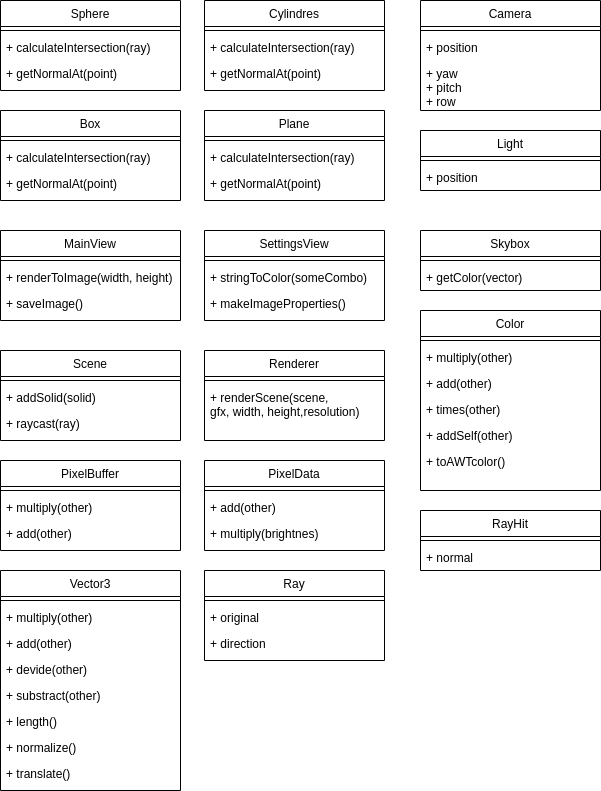
\includegraphics[width=0.8\textwidth]{assets/uml.png}
		\caption{Структура классов}
		\label{fig:class_diagram1}}
\end{figure}

\end{itemize}

\section{Интерфейс}

На рисунках \ref{img:inter-1} и \ref{img:inter-2} представлен интерфейс программы и настроек программы соответственно.

\begin{figure}[ht!]
	\centering{
		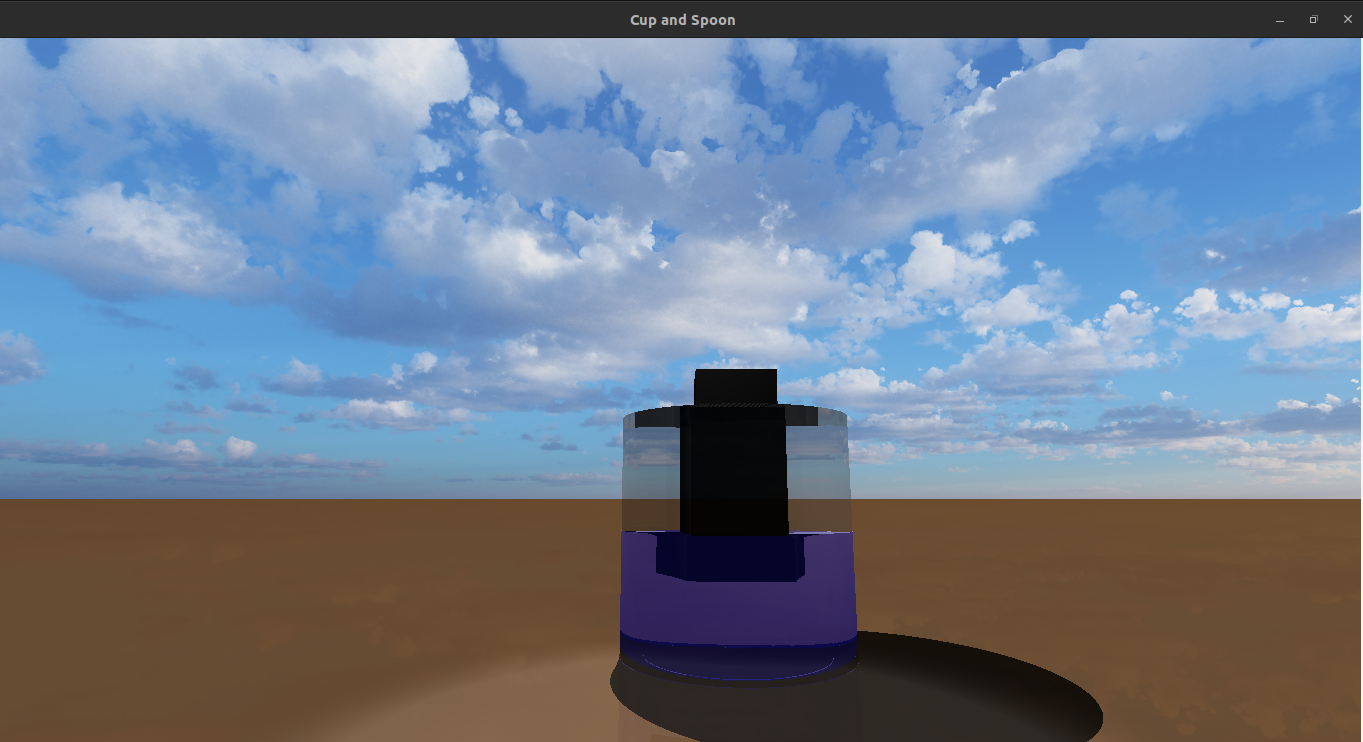
\includegraphics[width=0.8\textwidth]{assets/interface-1.png}
		\caption{Интерфейс программы}
		\label{img:inter-1}}
\end{figure}

\begin{figure}[ht!]
	\centering{
		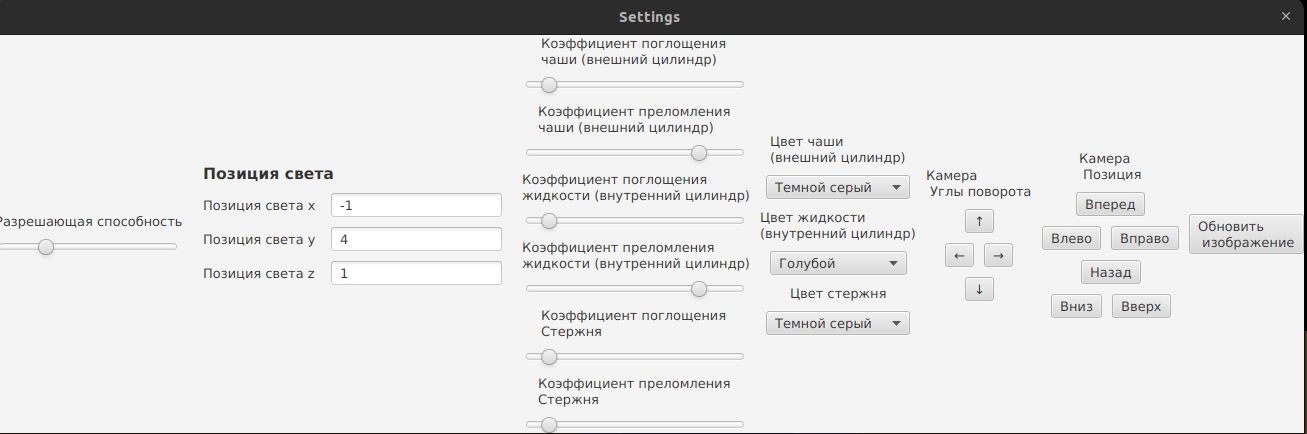
\includegraphics[width=0.8\textwidth]{assets/interface-2.png}
		\caption{Интерфейс настроек программы}
		\label{img:inter-2}}
\end{figure}

Функции представленных полей следующие:
\begin{itemize}
	\item полоса прокрутки <<Разрешающая способность>> --- изменение разрешающей способности выходного изображения;
	\item поля <<Позиция света>> --- задание положения источника света;
	\item полоса прокрутки <<Коэффициент поглощения емкости>> --- изменение коэффициента поглощения емкости;
	\item полоса прокрутки <<Коэффициент преломления емкости>> --- изменение коэффициента преломления емкости;
	\item полоса прокрутки <<Коэффициент поглощения жидкости>> --- изменение коэффициента поглощения жидкости;
	\item полоса прокрутки <<Коэффициент преломления жидкости>> --- изменение коэффициента преломления жидкости;
	\item полоса прокрутки <<Коэффициент поглощения параллелепипеда>> --- изменение коэффициента поглощения параллелепипеда;
	\item полоса прокрутки <<Коэффициент преломления параллелепипеда>> --- изменение коэффициента преломления параллелепипеда;
	\item всплывающее меню <<Цвет емкости>> --- изменение цвета чащи;
	\item всплывающее меню <<Цвет жидкости>> --- изменение цвета жидкости;
	\item всплывающее меню <<Цвет стержня>> --- изменение цвета стержня;
	\item кнопки <<Камера углы поворота>> --- изменение углов поворота камеры на 20 градусов в зависимости от выбранного направления;
	\item кнопки <<Камера позиция>> --- изменение положение камеры по координате в зависимости от выбранной кнопки;
	\begin{itemize}
		\item кнопка <<Вперед>> --- прибавление 1 к координате z;
		\item кнопка <<Назад>> --- вычитание 1 к координате z;
		\item кнопка <<Вправо>> --- прибавление 1 к координате x;
		\item кнопка <<Влево>> --- вычитание 1 к координате x;
		\item кнопка <<Вверх>> --- прибавление 1 к координате y;
		\item кнопка <<Вниз>> --- вычитание 1 к координате y;
	\end{itemize}
	\item кнопки <<Обновить изображение>> --- обновление изображения в зависимости от выбранных параметров;
\end{itemize}

\section*{Вывод}
В этом разделе был выбран язык программирования и среда разработки, рассмотрены роли основных классов, подробно разобран интерфейс приложения.
